\documentclass[
    DIV=11,
    BCOR=0mm,
    paper=a4,
    fontsize=11pt,
    % parskip=half,
    twoside=false,
    titlepage=true
% ]{scrreprt}
]{scrartcl}


% -- The basics
\setlength{\parskip}{0.5em} % What parskip=half would do in document class
\setlength{\parindent}{1em} % What would be indent if no parskip given in documentclass
% Set things manually, then we can have indent+skip

\usepackage[left=1in,right=1in,top=0.5in,bottom=1in]{geometry}
\usepackage{graphicx}
\usepackage[utf8]{inputenc}
\usepackage[ngerman, english]{babel}
\usepackage[expansion=true, protrusion=true]{microtype}


% -- Page setup
\usepackage[singlespacing]{setspace} 
\usepackage[automark, headsepline]{scrlayer-scrpage}
\clearmainofpairofpagestyles
\setlength{\headheight}{\baselineskip}
\automark{section} % write section in footline instead of chapter (if there is one)
\automark*{subsection}
\ihead{Max Melching \hfill \headmark}
\usepackage{lastpage}
\cfoot{{\hypersetup{linkcolor=black}Page~\thepage~of~\pageref{LastPage}}}


% -- Link setup
\usepackage{xcolor}
\definecolor{linkblue}{rgb}{0.00,0.00,1.00}

\usepackage{hyperref}
\hypersetup{
    colorlinks=true,
    breaklinks=true,
    citecolor=linkblue,
    linkcolor=linkblue,
    menucolor=linkblue,
    urlcolor=linkblue
}


% -- Font preferences
\usepackage{newtxmath}
\usepackage{tgpagella}
% \setkomafont{chapter}{\rmfamily\Huge\bfseries}
\setkomafont{section}{\rmfamily\Large\bfseries}
\setkomafont{subsection}{\rmfamily\large\scshape}
\setkomafont{paragraph}{\rmfamily}
\setkomafont{title}{\bfseries}
\setkomafont{subtitle}{\Large\scshape}
\setkomafont{author}{\Large\slshape}
\setkomafont{pagehead}{\scshape}
\setkomafont{pagefoot}{\slshape}


% -- Choose special color and font for code bits
\definecolor{codecolor}{RGB}{235, 66, 0}
\newcommand{\code}[1]{\textcolor{codecolor}{\texttt{#1}}}


% -- Customizing itemize labels
\renewcommand{\labelitemi}{$\blacktriangleright$}%{$\vartriangleright$}
\renewcommand{\labelitemii}{\textbf{--}} % is also default there
\renewcommand{\labelitemiii}{$\bullet$}
\setlength{\itemsep}{10pt}


% -- Retrieving git hash
\usepackage{xstring}
\usepackage{catchfile}
\CatchFileDef{\HEAD}{.git/refs/heads/main}{}
\newcommand{\gitrevision}{%
  \StrLeft{\HEAD}{7}%
}
% \CatchFileDef{\TAG}{.git/refs/tags}{}


% -- Some convenience features
\usepackage{siunitx}
\usepackage{wasysym}  % For \ascnode symbol


% -- Some custom commands
\newcommand{\defaultval}[1]{%
    {\bfseries\slshape%\itshape
    % Default:} #1%
    Default} $=$ #1%
}


\usepackage{xspace}
\def\tikzfancy{Ti\textit{k}z\xspace}



\begin{document}



{\noindent\rmfamily\Huge\bfseries
    Documentation Of \code{GWFrames}
}

\begin{center}
    \textbf{Contact:} consider opening a \href{https://github.com/MaxMelching/minkowski_diagram/issues}{GitHub issue} or find me at \href{mailto:m-melching@web.de}{m-melching@web.de}.
\end{center}


For the most recent version of all the files, see \url{https://github.com/MaxMelching/gw_frames}.
This file was compiled on \today{} and the corresponding git commit hash
is \code{\gitrevision{}} (or, in case you need the full one, \code{\HEAD{}}\hspace{-0.5em}).



    \section{Overview}

This repository contains three packages, each providing one command:
\begin{itemize}
    \item \code{cbc\_frames\_tikz} (command \verb|\drawframes|): plots a
    selection of source frame, signal frame, and celestial frame that are
    used to describe gravitational waves emitted by compact binary coalescences.
    
    
    \item \code{cbc\_binary\_tikz} (command \verb|\drawbinary|): plots
    intrinsic parameters of a system of two compact binary objects. Adapted
    from code originally written by Jannik Mielke.
    
    
    \item \code{earth\_tikz} (command \verb|\drawearth|): plots one side of
    the Earth. Mainly intended for usage through \verb|\drawframes|. Most of
    the credit for this code goes to Izaak Neutelings, who provided it on
    \url{https://tikz.net/astronomy_seasons/}.
\end{itemize}

Several examples of how to use this package are shown in the examples folder.
% Pictures are also included in Fig.~\ref{fig:examples}.

% \begin{figure}[h]
%     \centering

%     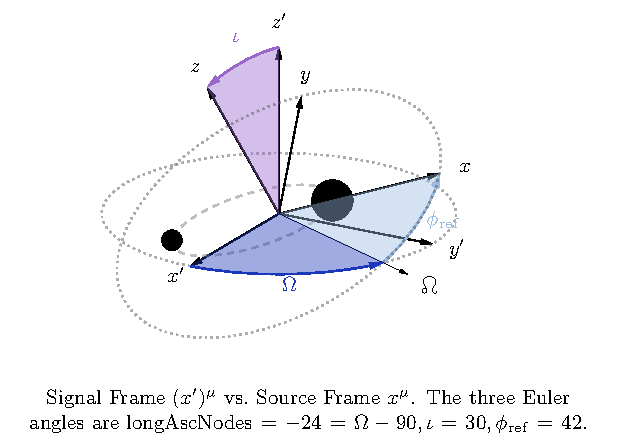
\includegraphics[width=0.67\textwidth]{examples/signal_frame.pdf}
%     \label{fig:examples}
% \end{figure}



    \section{List Of Keyword Arguments}

\emph{Note} that certain values cannot be passed to pgfkeys, which is
particularly relevant for declaration of labels. If you encounter an issue of
this kind, look up the command that this key is stored in (typically something
like \verb|\<parameter>Label|), and manually set the command. This can be done
using \verb|\def\<parameter>Label{<input>}|. A practical example would be
\verb|\def\OmegaLabel{$\Omega = \pi/2 + \mathrm{longAscNodes}$}|.



        \subsection{\texttt{cbc\_frames\_tikz}}
This is a list of all keyword arguments (note that all angles are expected to
be given in degrees):
\begin{itemize}
    \item \code{mass1}: Mass of the first compact object, determining its size. Ten solar masses correspond to a size of $\SI{0.35}{\centi\metre}$.

    \defaultval{$20$}


    \item \code{mass2}: Mass of the second compact object, determining its size. Ten solar masses correspond to a size of $\SI{0.35}{\centi\metre}$.

    \defaultval{$20$}


    \item \code{inclination}: Inclination between orbital plane and sky plane. This rotation is about the ascending node $\ascnode$.

    \defaultval{$0$}


    \item \code{polarization}: Polarization angle, i.e. rotation of the $x$-axis in the sky plane (about the line of sight, which coincides with the $z$-axis of the signal frame).

    \defaultval{$0$}


    \item \code{longascnodes}: Determines the ngle between $x$-axis of the signal frame and the ascending node $\ascnode$, which is $\Omega = 90 + \mathrm{longAscNodes}$.

    \defaultval{$0$}


    \item \code{phiref}: Reference angle $\phi_\mathrm{ref}$ that determines the rotation between ascending node and $x$-axis of the signal frame (about the inclined $z$-axis of the signal frame).

    \defaultval{$0$}


    \item \code{ra}

    \defaultval{$0$}


    \item \code{dec}

    \defaultval{$0$}


    \item \code{eccentricity}: Determines the circularity of the binary black hole orbit

    \defaultval{$0$}


    \item \code{axislen}: Length of the axes of each coordinate system.

    % \defaultval{$\SI{3}{\centi\metre}$}
    \defaultval{$3$}


    \item \code{axislabelpad}: How far from the axis label is drawn from the axis arrow tip, in multiples of \code{axislen}.

    \defaultval{$0.12$}


    \item \code{binaryscalefactor}: Distance of binary companions, in multiples of \code{axislen}.

    \defaultval{$0.5$}


    \item \code{binarydistance}: distance of binary center of mass from Earth, in multiples of the axis length \code{axislen}.

    \defaultval{$3$}


    % \item \code{uselayers}


    \item \code{showcelestialframe}: Whether to show the celestial frame. Has precedence over the other commands for the styling of the celestial frame, such as \code{celestialframeaxes}.

    \defaultval{true}


    \item \code{celestialframeaxes}: Whether to show the celestial frame axes.

    \defaultval{true}


    \item \code{celestialframehelperlines}: Whether to show the celestial frame helper lines.

    \defaultval{true}


    \item \code{celestialframeangles}: Whether to visualize the celestial frame angles.

    \defaultval{true}


    \item \code{showlineofsight}: Whether to visualize the line of sight (and accordingly, the luminosity distance).

    \defaultval{true}


    \item \code{showsignalframe}: Whether to show the signal frame. Has precedence over the other commands for the styling of the signal frame, such as \code{signalframeaxes}.

    \defaultval{true}


    \item \code{signalframeaxes}: Whether to show the signal frame axes.

    \defaultval{true}


    \item \code{signalframehelperlines}: Whether to show the signal frame helper lines.

    \defaultval{true}


    \item \code{signalframeangles}: Whether to visualize the signal frame angles.

    \defaultval{true}


    \item \code{showsourceframe}. Whether to show the source frame. Has precedence over the other commands for the styling of the source frame, such as \code{sourceframeaxes}.

    \defaultval{true}


    \item \code{sourceframeaxes}: Whether to show the source frame axes.

    \defaultval{true}


    \item \code{sourceframehelperlines}: Whether to show the source frame helper lines.

    \defaultval{true}


    \item \code{earthradius}: Radius of the Earth that is drawn as part of the celestial frame. Passed on the \code{radius} argument of \code{earth\_tikz}.

    \defaultval{$1.25$}


    \item \code{earthtilt}: Tilt of the Earth that is drawn as part of the celestial frame. Passed on the \code{radius} argument of \code{earth\_tikz}.

    \defaultval{$0$}


    \item \code{showifo}: Whether to draw an interferometer on Earth.

    \defaultval{true}


    \item \code{ifoarmlength}: Arm length of the interferometer.

    % \defaultval{$\SI{2}{\centi\metre}$}
    \defaultval{$2$}


    \item \code{showazimuthalangle}: Determines if a specific azimuthal angle used in [this](https://www.nature.com/articles/s41550-025-02632-5) paper is visualized.

    \defaultval{false}
\end{itemize}



        \subsection{\texttt{cbc\_binary\_tikz}}
\begin{itemize}
    \item 
\end{itemize}



        \subsection{\texttt{earth\_tikz}}
\begin{itemize}
    \item \code{radius}: Radius of the Earth
    
    \defaultval{$1$}


    \item \code{tilt}: Tilt of the Earth
    
    \defaultval{$0$}
\end{itemize}



\end{document}